\chapter{实验环境}
\section{模型设计}
考虑在具有多种可调度资源的单个服务器上混合执行延迟敏感型任务和批处理任务的问题。智能体执行调度的周期可设置为足够小,以至于在每个时间步骤内,延迟敏感型任务的负载可视为基本不发生变化。通过调度决策开始时到延迟敏感型应用的请求数量,可以预计此段时间步骤内延迟敏感型任务的负载强度。根据预计的负载强度和当前服务器的各类资源利用率(环境状态),智能体选择动作进行资源调度。在当前周期结束后,智能体将收到新的预计负载强度和新的服务器资源利用率。同时,智能体还会收到反映上一个动作质量的奖励信号。

智能体的优化目标是在不违反延迟敏感型任务的服务质量要求的同时,优化服务器的资源利用率。当我们假设批处理任务可以充分利用被分配的资源时,一个相关的且容易量化的优化目标为分配给延迟敏感型任务的资源尽量少。上述假设通常是成立的。

\subsection{隔离技术}
\textbf{计算核心资源}直接影响任务获得的计算速度和并行计算能力。通过Linux系统提供的cgroup,我们可以任意为延迟敏感型任务和批处理任务分配计算核心。实验在英特尔Xeon(R
) E5-2630上进行。该处理器具有10个物理计算核心,20个逻辑计算核心。英特尔的超线程技术使得共用同一个物理计算核心的超线程将共用一二级高速缓存。而对于非末级高速缓存的访问目前没有办法进行隔离,因此我们将资源分配的粒度设置为分配物理核心以防止批处理任务与延迟敏感型任务在同一物理核心上运行时在一二级高速缓存上产生干扰。\textbf{末级高速缓存}上批处理任务对延迟敏感型任务在延迟敏感型任务高负载强度时产生巨大的干扰。因此隔离任务对末级高速缓存的使用能有效保证延迟敏感型任务在高负载强度时的服务质量。处理器硬件提供20级的缓存分配,为简化问题,我们将缓存分配设置为10级,即资源分配的粒度为末级高速缓存总大小的十分之一。用于控制\textbf{动态随机存储访问带宽}的内存带宽分配技术(MBA)在实验环境的服务器上缺乏硬件支持,因此无法直接控制混合执行任务对动态随机存储器的访问。
用于替代内存带宽分配技术,我们一般通过内存带宽监控技术(MBM)检测每个计算核心产生的动态随机存储访问流量,当批处理任务对动态随机存储访问带宽产生过大压力时,减少分配给批处理任务的计算核心以降低其对动态随机存储的访问,然而从后续一节\nameref{sec:pref_analysic}中发现,这种粗粒度的调节并不能取得很好效果。

\begin{figure}
  \centering
    \centering
    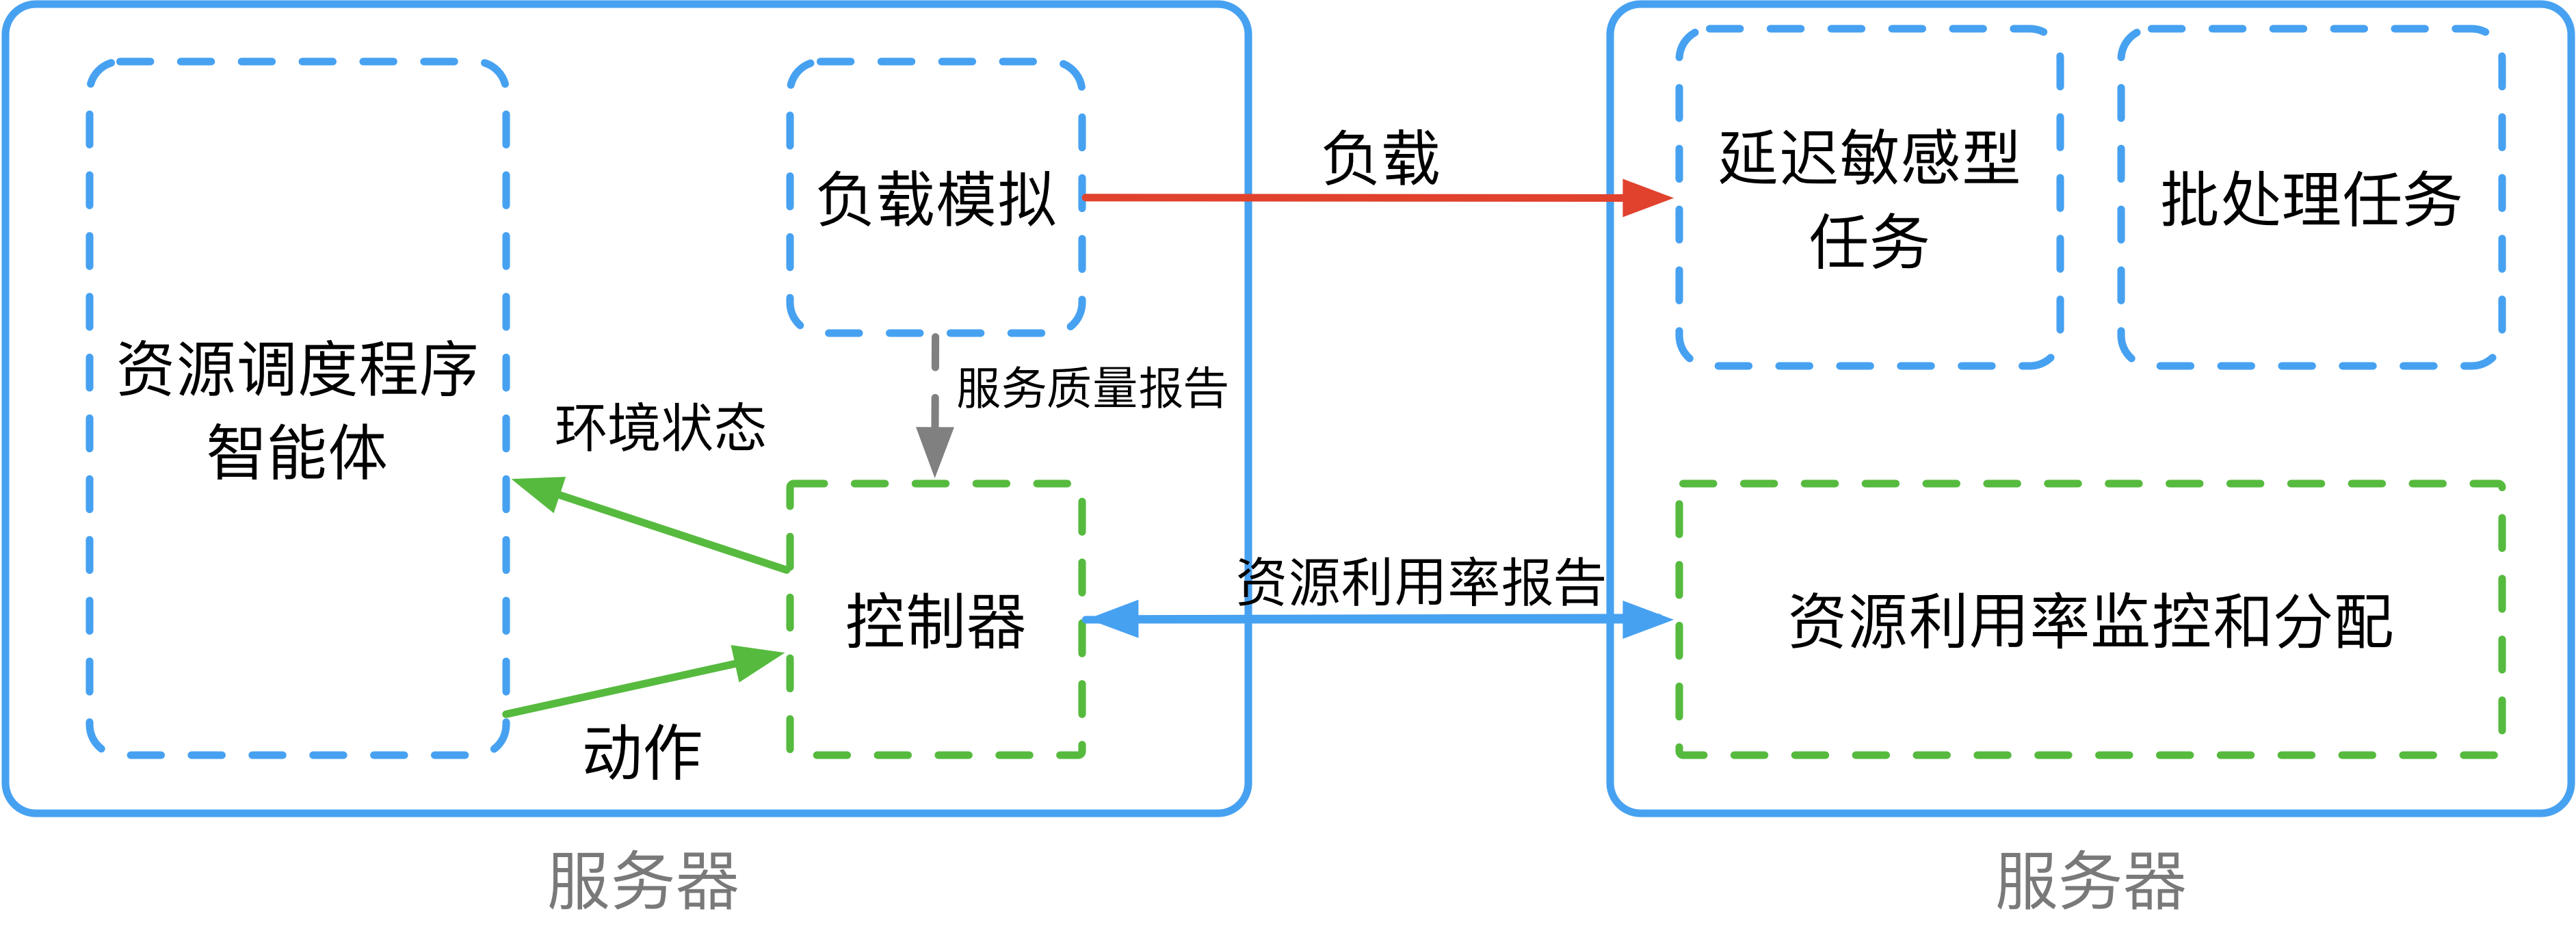
\includegraphics[width=0.9\linewidth]{exp/overview.png}
    \captionof{figure}{实验系统架构}
    \label{fig:overview}    
\end{figure}

\subsection{整体架构}
为避免资源调度算法与延迟敏感型程序抢夺资源,资源调度程序将在单独的硬件上运行,并通过与延迟敏感型程序混合执行的一个轻量控制程序监控资源利用和进行资源调度。系统的整体架构如图\ref{fig:overview}所示。

充当资源调度程序的智能体通过与其运行在同一服务器上的控制器与环境交互。当只能体做出动作时,控制器接受智能体的动作,并将其传递至被调度服务器上执行。被调度的服务器上运行的轻量控制器将在指定的时间内取样服务器的资源利用率并返回给调度程序端的控制器。除了执行来自智能体的动作,控制器还将调动负载模拟程序向延迟敏感型任务施加负载并收回此段时间内的服务质量报告。为了获得具有统计学意义的数据,以上施加负载和采样资源利用率的过程都被设定为足够长以允许延迟敏感型任务服务足够多的请求。所有搜集到的数据,包括资源利用率报告和服务质量报告,将作为环境状态和计算出的此步骤奖励一起返回给资源调度智能体。

\section{混合执行任务选择}
\subsection{延迟敏感型任务}
数据中心常见的延迟敏感型任务包括社交网络,搜索引擎,软件即服务,在线地图,网页邮箱,机器翻译,在线购物和广告等等。

\subsubsection{Elgg 社交服务引擎}\lable{sec:elgg}
社交网络应用与普通网站服务不同,其更多是一个平台。例如脸书(Facebook)就给用户提供了一个社交平台。社交网络上的大部分数据是由用户(而不是开发者)产生。这些数据由其他用户的行为,或外来资源的变化而引起动态更新,并被推送给用户。正因为如此,社交网络应用包含频繁的后端数据库写入,且写入的数据将在后来推送给用户。

Elgg社交服务引擎是一个基于PHP实现的开源社交网络应用,并被包括澳大利亚政府,新西兰教育部,Wiley出版社,弗罗里达大学在内的机构使用\cite{palit2016demystifying}。Elgg社交服务引擎提供与流行的社交服务脸书提供相似的功能,允许用户在其中建立一个个人好友网络,并在网络中互相分享内容。Elgg社交引擎还包括一个迷你博客Elgg Wire,可用于与其他用户分享文字,图片和视频内容。在Elgg Wire中分享的内容被其他用户可见,类似与脸书中发文上墙的功能。每一个用户都有自己的实时与好友网络共享的信息流,被称为Elgg River。通过Elgg,用户可以实现多种操作,比如发送和接收聊天信息,在Elgg Wire上发送动态,以及接收其他用户最新分享的内容。所有的操作都有AJAX发送和接受简短消息实现,因此Elgg的主要负载都是这些来自AJAX的简短请求。

Elgg的后端通过服务器脚本语言PHP和MySQL数据库实现。脸书的服务器后端相似\cite{nishtala2013scaling},我们还通过Memcached加速数据库访问。为了简化问题,Elgg的网页服务器和后端,包括MySQL和Memcached都运行在同一服务器上,并作为延迟敏感型任务分配资源。

我们使用Faban框架来实现Elgg社交引擎的服务质量测试。Faban是一个基于Java的基准测试开发和执行框架,提供了API用于快速开发基准测试程序。通过定义测试的操作和各种操作的执行概率,可以快速开发网络应用的基准测试。在基准测试完成后,Faban将输出各个操作执行情况的统计数据,例如执行测试,相应时间和违反服务质量要求的情况。

Elgg提供了多种功能,因此用户可以进行多种操作,例如登录登出,添加好友,发送接收消息和分享动态等。考虑到真实用户执行不同操作具有不同频率,且每一个操作与前一个操作具有一定关联,我们通过一个马尔科夫过程(Markov Process)模拟用户的行为。Elgg的服务质量被定义为一段时间内所有该操作的响应时间的九十分位点。从服务器来看,模拟用户总体的产生的各个操作的比例各个操作和其服务质量要求如表\ref{tab:mix}所示。对于Elgg引擎服务质量的设置参考于Facebook各操作的平均延迟\cite{alexa2016},对于注册、登录和退出等用户不频繁使用的的操作,设置了较低的服务质量要求。

\begin{table}[!htp]
  \centering
  \captionof{table}{模拟用户总体访问模式}\label{tab:mix}
  \begin{tabular}{@{}lcc|lcc|lcc@{}} \toprule
    操作 & 占比 & 服务质量要求 & 操作 & 占比 & 服务质量要求 & 操作 & 占比 & 服务质量要求\\ 
    \midrule
    注册 & 0.5 & 3 & 首页 & 5 & 1 & 发消息 & 17 & 1 \\
    登录 & 2.5 & 3 & 动态 & 20 & 1 & 收消息 & 17 & 1 \\
    退出 & 2.5 & 3 & 好友 & 10 & 1 & 刷新主页 & 25.5 & 1\\
    \bottomrule
  \end{tabular}  
\end{table}

\subsubsection{对象缓存服务}
为了提高性能,网络应用通常使用对象缓存服务(Object Caching)来缓存一些代价昂贵的操作的计算结果,因此对象缓存服务存储和读取的速度将极大影响整个服务的性能。Memcached是一个常用的以键—值形式存储的对象缓存系统,通常用来缓存一些用时较长的数据库请求的结果。对网页服务器的一个请求一般会使网络服务器产生多个对对象缓存服务的请求。为了避免网页加载的延迟,对象存储服务必须以低延迟返回请求结果,因此其服务质量(九十分位延迟)通常设置在十毫秒。

Cloudsuit中提供了Memcached的基准测试程序Memloader\cite{palit2016demystifying}。由于对象缓存服务的请求基本无需额外的处理,因此对象缓存服务器除了低延迟外,还具有很高吞吐量。Memloader对此优化了基准测试程序结构。测试程序通过C++实现以提高性能,在其产生的多个测试线程中,一半的线程进行请求,另一边的线程验证缓存服务返回的信息。两种线程的分工减少了请求和处理间的干扰,有利于准确计时和产生统计信息。由于Memcached已知的规模扩展问题,即当其产生超过四个线程时会由显著性能下降,因此实践中一般在一个服务器上运行多个Memcached实例。Memloader可以在多个缓存服务器之间平衡负载。测试结束后,基准测试可以报告平均的请求延迟,九十分位延迟和缓存命中率等数据。

Memcached的高吞吐量使得缓存服务器和运行基准测试的服务器之间的网络连接成为性能瓶颈,通常要求其间的连接带宽在10Gbps以上。实验环境中不具备这样的网络连接条件,为避免网络瓶颈,我们在具有多个处理器接口的服务器上,每个接口分别运行对象缓存服务和基准测试程序,以利用系统中高速的网络回路连接(loopback)。

\subsection{批处理任务}
数据中心存在多种批处理任务,例如文件备份,离线图片处理和视频转码压缩等。来自普林斯顿大学的测试程序套装(Princeton Application Repository for Shared-Memory Computer, PARSEC)\cite{bienia11benchmarking}包含了一些典型的数据中心批处理任务。

\subsubsection{视频编码}
随着存储和网络带宽的增加,网络视频在网络流量中占比显著增加,视频的解码,转码,压缩等任务对于如Youtube的视频网站十分重要。视频编码测试程序parsec.x264是一个基于H264/AVC(Advanced Video Coding)标准的视频编码器,用于将图像有损压缩为一个视频流。与前一代视频编码标准相比,H264可以以更低比特率输出高质量视频,也因此成为了包括视频会议和视频分发等应用的常用标准。然而H264的高压缩率通过更多的转码和解码计算得来,因此相比上一代标准,编码和解码H264需要更强的计算能力。

H264编码器和解码器操作在固定的,大小为16乘16的像素块内。多种技术被运用其中以检测和减少数据冗余。其中最重要的技术是运动补偿(Motion Compensation)。动作补偿被应用在连续帧之间以检测每帧图像时间时间上的冗余。动作补偿对最后视频的压缩率有决定性作用,但同时也是压缩视频流时运算量最大的操作。H264编码器输出的帧有三种类型,I类,P类和B类(I-frame, P-frame,B-frame),且每一帧输出对前后一帧输出都有依赖。parsec.x264应用通过流水线并行,其结果之间相互依赖的性质导致其大量的进程间通信,因此共享高速缓存的容量对其性能有较大影响。x264的大量数据输入输出量,也会对共享高速缓存和动态随机存储器的访问带宽造成较大影响。图\ref{fig:batch_cache}(a)表示了缓存大小对x264的缓存未命中率的影响\cite{bienia2008parsec}。

\begin{figure}
  \centering
  \begin{subfigure}{0.4\textwidth}
    \centering
    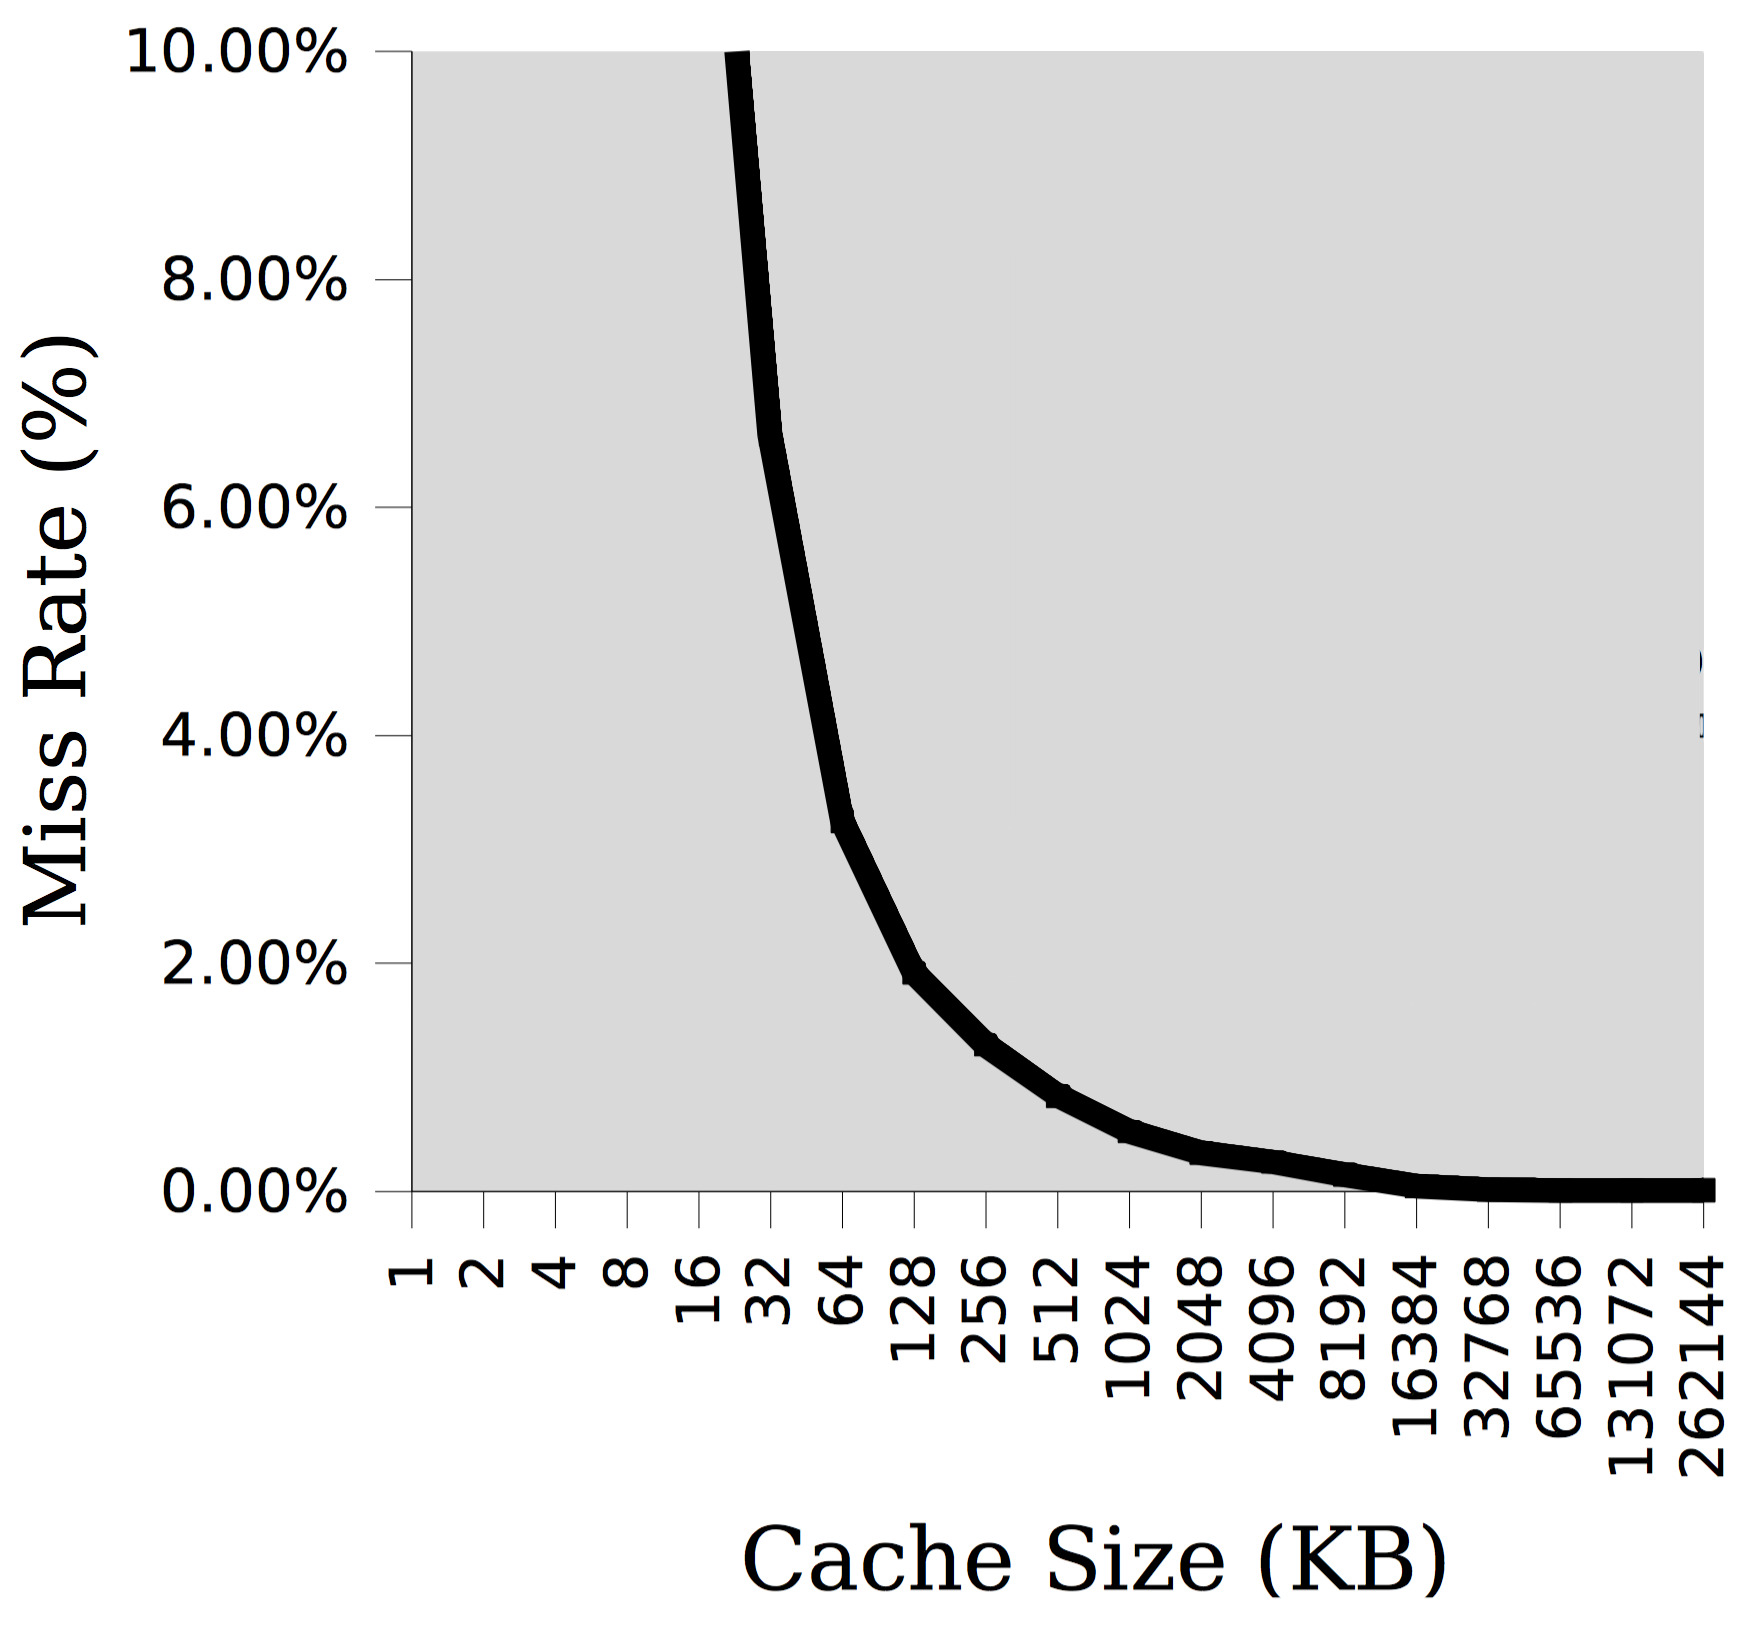
\includegraphics[height=6cm]{exp/x264.png}
    \captionof{figure}{PARSEC.x264}
  \end{subfigure}
  \hspace{4em}
  \begin{subfigure}{0.4\textwidth}
    \centering
    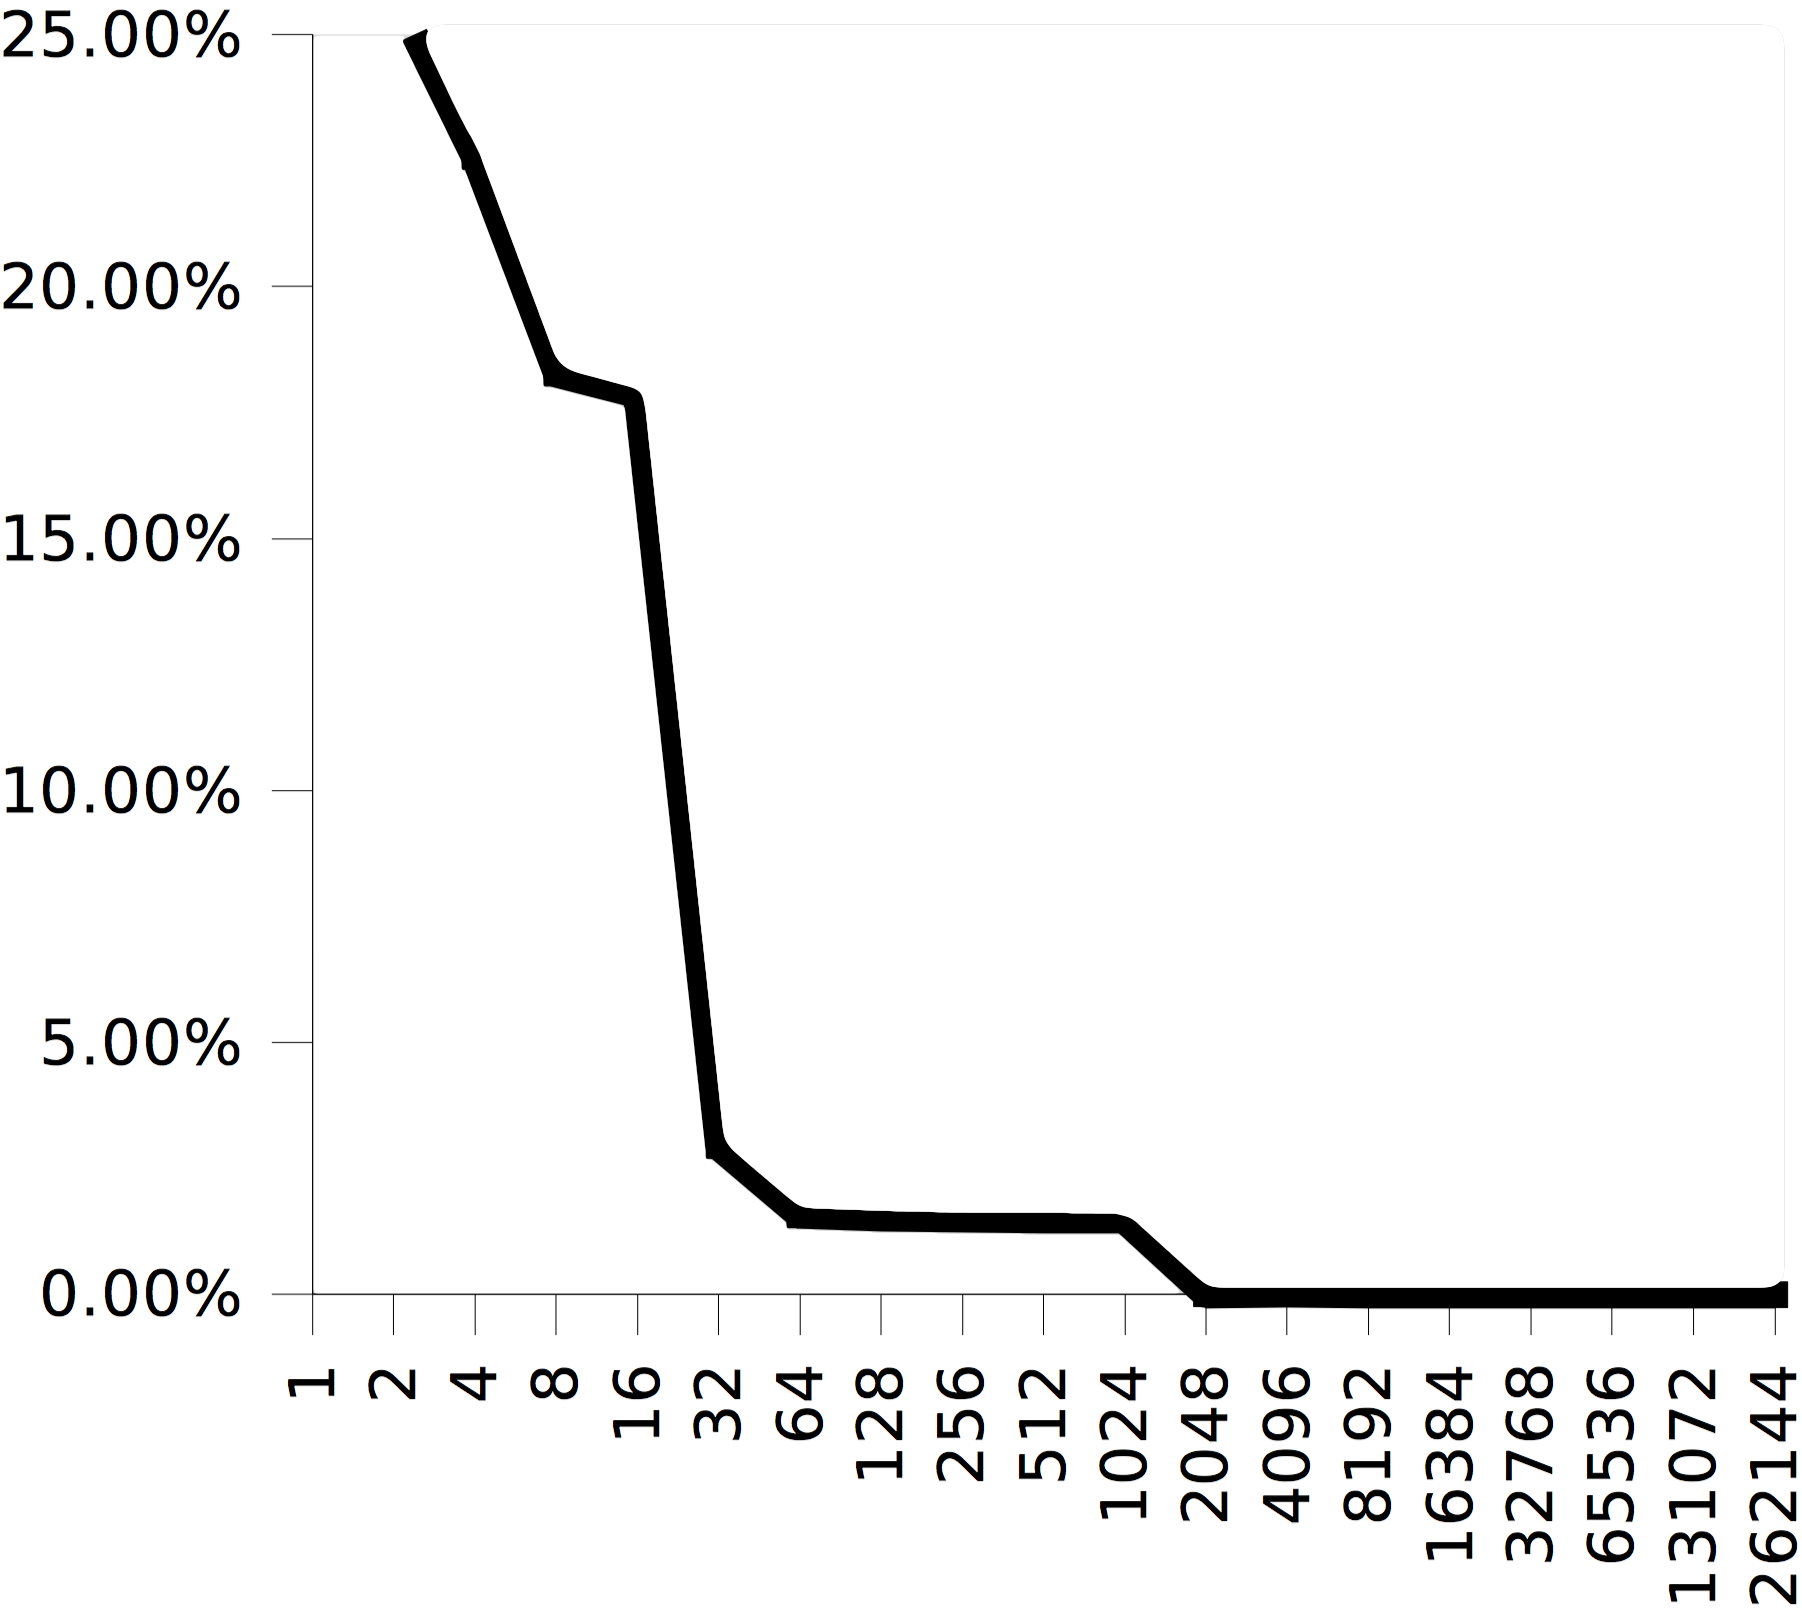
\includegraphics[height=6cm]{exp/blackschole.png}
    \captionof{figure}{PARSEC.BlackScholes}
  \end{subfigure}
  \captionof{figure}{批处理任务的缓存未命中率与缓存容量}
  \label{fig:batch_cache}
\end{figure}
\subsubsection{期权定价}
Parsec中包含一个基于布莱克-舒尔斯(Black-Scholes)等式的欧式期权定价应用。布莱克-舒尔斯等式是一个偏微分方程,且没有一个解析解,因此必须通过数值计算的方法找到其近似解。此应用金融工程中大量的偏微分方程求解认为的代表。应用并行求解多个方程,需要进行大量的浮点数计算。由于其所需求的数据量量较少,因此对缓存和内存系统的压力较小,如图\ref{fig:batch_cache}(b)。

\section{任务资源需求分析}\label{sec:pref_analysic}
Elgg社交服务引擎在与parsec.x264任务混合执行时,给定十个逻辑内核(50\%,总共二十个逻辑内核)和50\%的末级高速缓存,测得其各操作的服务质量性能(黑线)如图\ref{fig:latency}所示。实验中仅统计常用的操作,如收发消息和更新动态等;不常用的操作如注册,登录和退出等,在15秒采样时间内仅能取得少量样本,缺乏统计学意义,因此不予统计。所有统计的操作的服务质量的计量标准均为采样时间内响应时间的九十分位点,服务质量要求为响应时间的九十分位点不大于一秒(红线)。图中同时给出了其访问延迟的平均值(蓝线)和标准差(淡橙色方块)。
\vspace{1em}
\begin{figure}[h!]
  \centering
    \centering
    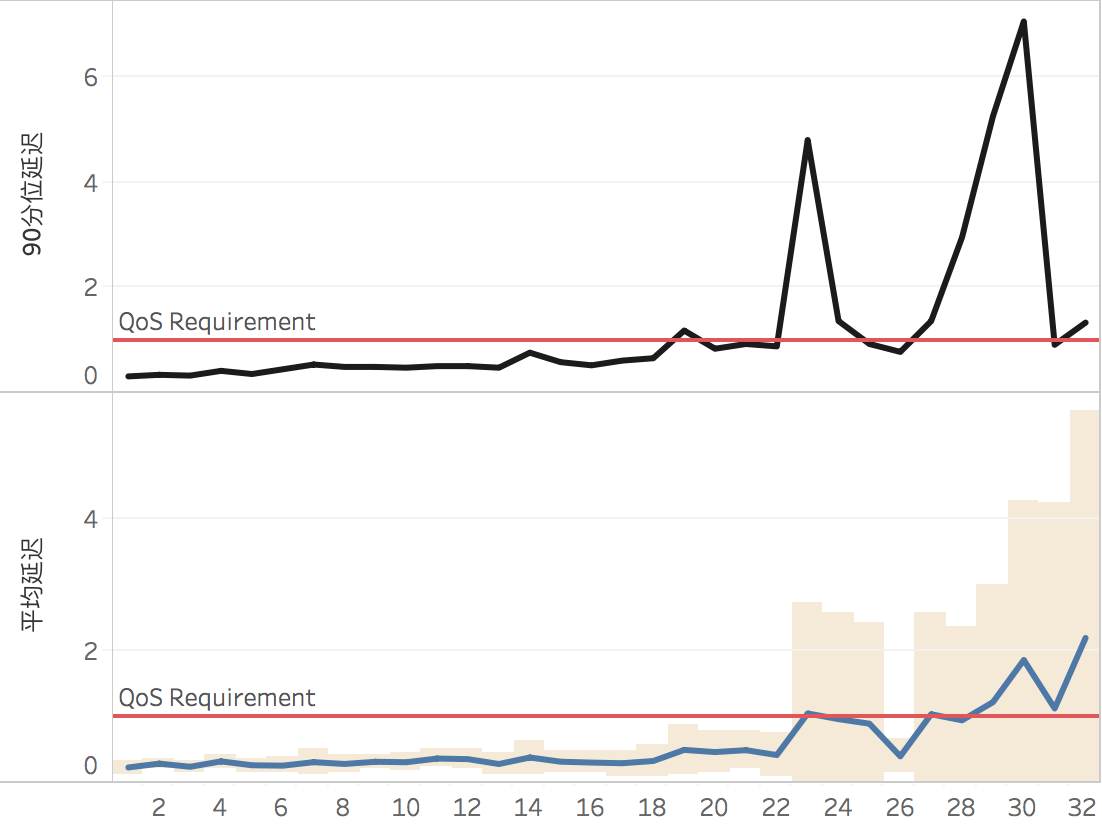
\includegraphics[width=0.85\linewidth]{exp/latency.png}
    \captionof{figure}{Elgg引擎的服务质量与负载强度}
    \label{fig:latency}    
\end{figure}

从图\ref{fig:latency}可以看到在负载强度较低时(用户数量在1至18内),Ellg社交引擎的平均延迟缓慢的上涨,且方差较小,上升趋势稳定,没有违反服务质量要求;在负载强度较高时(18至22),平均延迟的增长速度变快,方差变大,出现违反服务质量要求的情况;当负载强度严重超过在此时资源分配可承载的强度时(用户数量22-32),平均延迟迅速上升,方差显著变大,不但出现违反服务质量的要求,且性能表现不稳定。性能表现不稳定的原因可以部分归结在测试执行的方法。在实验的测试方法中,模拟用户线程启动后将各自登录并在登录后,按照\fullref{sec:elgg}所述的模式开始访问。测试程序将在模拟用户线程启动运行一段时间后开始采样。在Elgg社交引擎所获得的服务器资源严重不足以支持当前负载强度时,用户的登录操作可能反复失败引起后续的操作无法正常进行。另一方面,因服务器各个操作的访问延迟显著上升,采样开始后存在的大量的请求无法在采样时间内结束,进而无法统计其操作延迟。各个操作的相互影响使得服务器的服务质量变化巨大。可以肯定的一点是,在此种情况下,Elgg社交引擎显然违反了其服务质量要求。

\begin{figure}
  \centering
  \begin{subfigure}{0.4\textwidth}
    \centering
    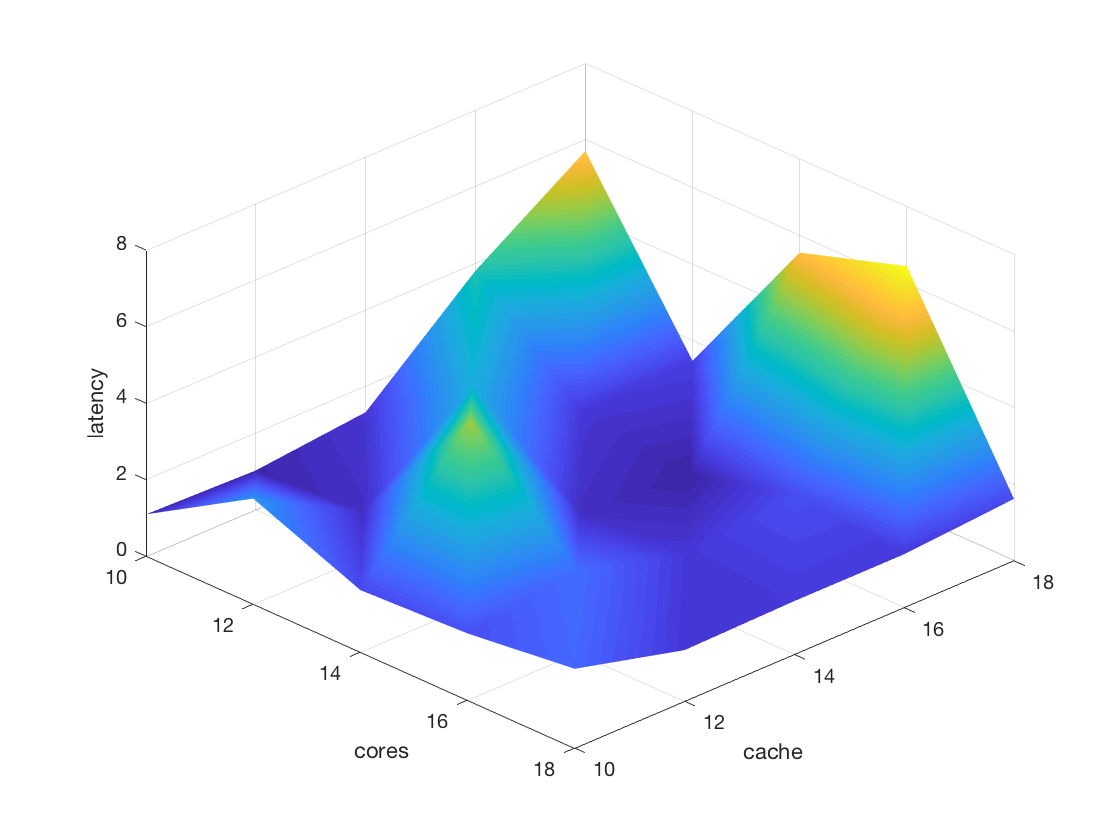
\includegraphics[height=6cm]{exp/fixed_load_var_resource.png}

  \end{subfigure}
  \hspace{3em}
  \begin{subfigure}{0.5\textwidth}
    \centering
    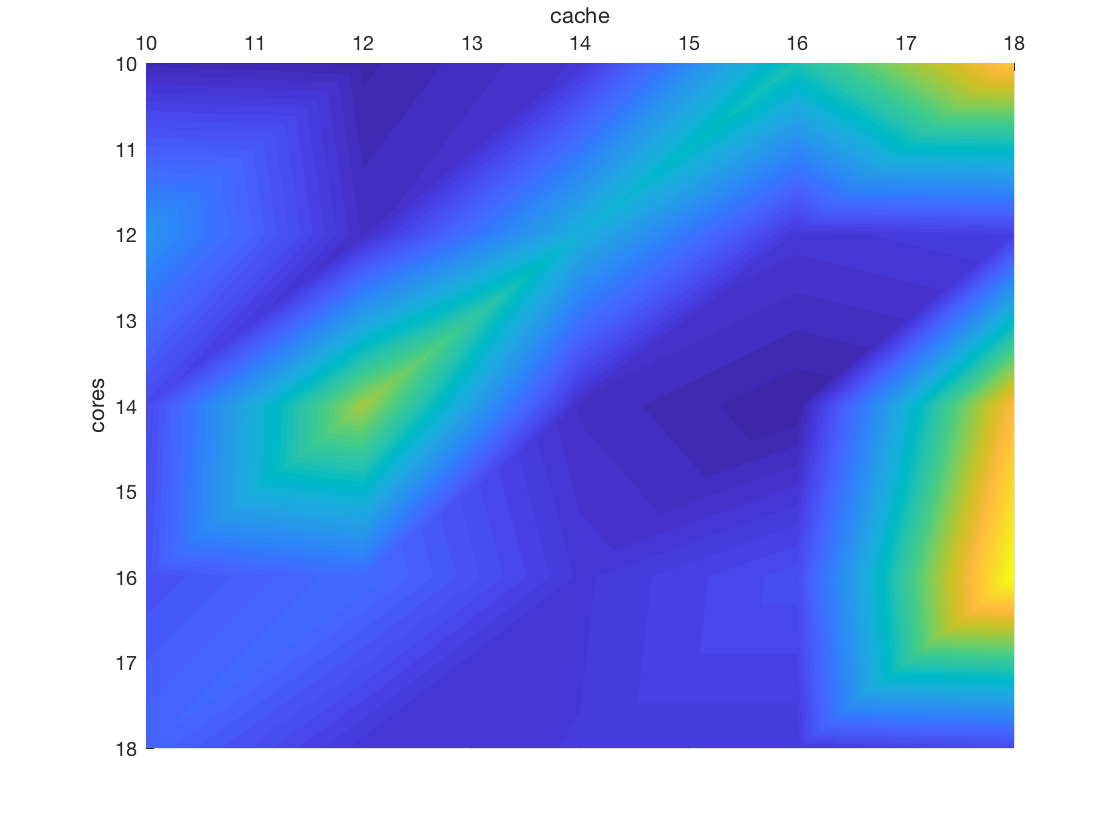
\includegraphics[height=6cm]{exp/fixed_load_var_resource_flat.png}

  \end{subfigure}
  \captionof{figure}{Elgg引擎的服务质量与服务器资源分配}
  \label{fig:fixed_load_var_resource}
\end{figure}

然而,这无法解释在高强度负载强度,Elgg持续违反服务质量要求时,出现性能的突然提高(模拟用户数量26)。图\ref{fig:fixed_load_var_resource}展示了Elgg引擎的服务质量与服务器资源分配关系的测试结果。首先容易看到,Elgg引擎的服务性能对计算核心数目与缓存大小并不敏感。Elgg服务的主要耗时在于数据库操作,存储用户发布都动态和查询用户好友发布的动态,因此其对缓存不敏感容易理解。同时,在为Elgg引擎分配大量缓存时,与之并行执行的批处理任务缓存容量受限产生大量的缓存不命中,进而大量占用内存带宽,干扰Elgg的数据库读写操作。因此,可以相信Elgg服务性能的对计算核心个数的不敏感,可以归结为内存访问带宽处的性能瓶颈。图\ref{fig:fixed_load_var_resource}右,可以看到其上一条斜45度向下的延迟高峰,其中的数据是通过每次固定核心个数,改变分配的缓存容量测得的。每次的测试用时相近,由此可以推断高峰出现具有固定周期。我们认为这样的周期性高延迟来自批处理任务周期性的读写数据高峰的硬性,这样的推断同时可以解释图\ref{fig:latency}中性能的剧烈变化。综上所述,parsec.x264过度的内存访问带宽导致了Elgg引擎的低性能。

由于缺少硬件支持的内存访问带宽隔离技术,我们只能通过限制x264运行的核心数来试图控制其带宽。x264应用具有高度的并行执行和各进程指令高度同步的特点。当出现内存访问高峰时,几乎所有进程将同时处于读取或写入内存的阶段。即使将多个这样的进程限制在同一核心,一个进程执行访问内存指令并阻塞后,下一进程也将被切换进计算核心执行。其内存访问无法通过控制计算核心数目得到有效控制,所以在Elgg社交服务引擎在与parsec.x264任务混合执行时,Elgg的服务质量难以保证。

由此看出,即使在存在资源隔离的条件下,通过一定手段(比如气泡测试\cite{mars2011bubble})合理的选择混合执行的任务也仍然重要。Memcached对象缓存服务具有每秒处理大量的请求(十万级),对计算核心数目有很高要求,且其对缓存容量敏感程度不高。parsec.black-scholes需要进行大量的浮点运算因此能有效利用空闲的计算核心,其大小始终的数据集不会对Memcached服务产生过大的压力。上述任务的混合可有效利用服务器资源,且容易对其产生的相互干扰进行细粒度的调控,因此是一个理想的任务混合方案。对象缓存服务在单独执行与混合执行的服务质量随资源分配的变化如图\ref{fig:data-cache-res}。可以看出,资源隔离技术在此有效的保证了延迟敏感型任务服务质量的稳定。
  \vspace{1em}
\begin{figure}
  \centering
  \begin{subfigure}{0.45\textwidth}
    \centering
    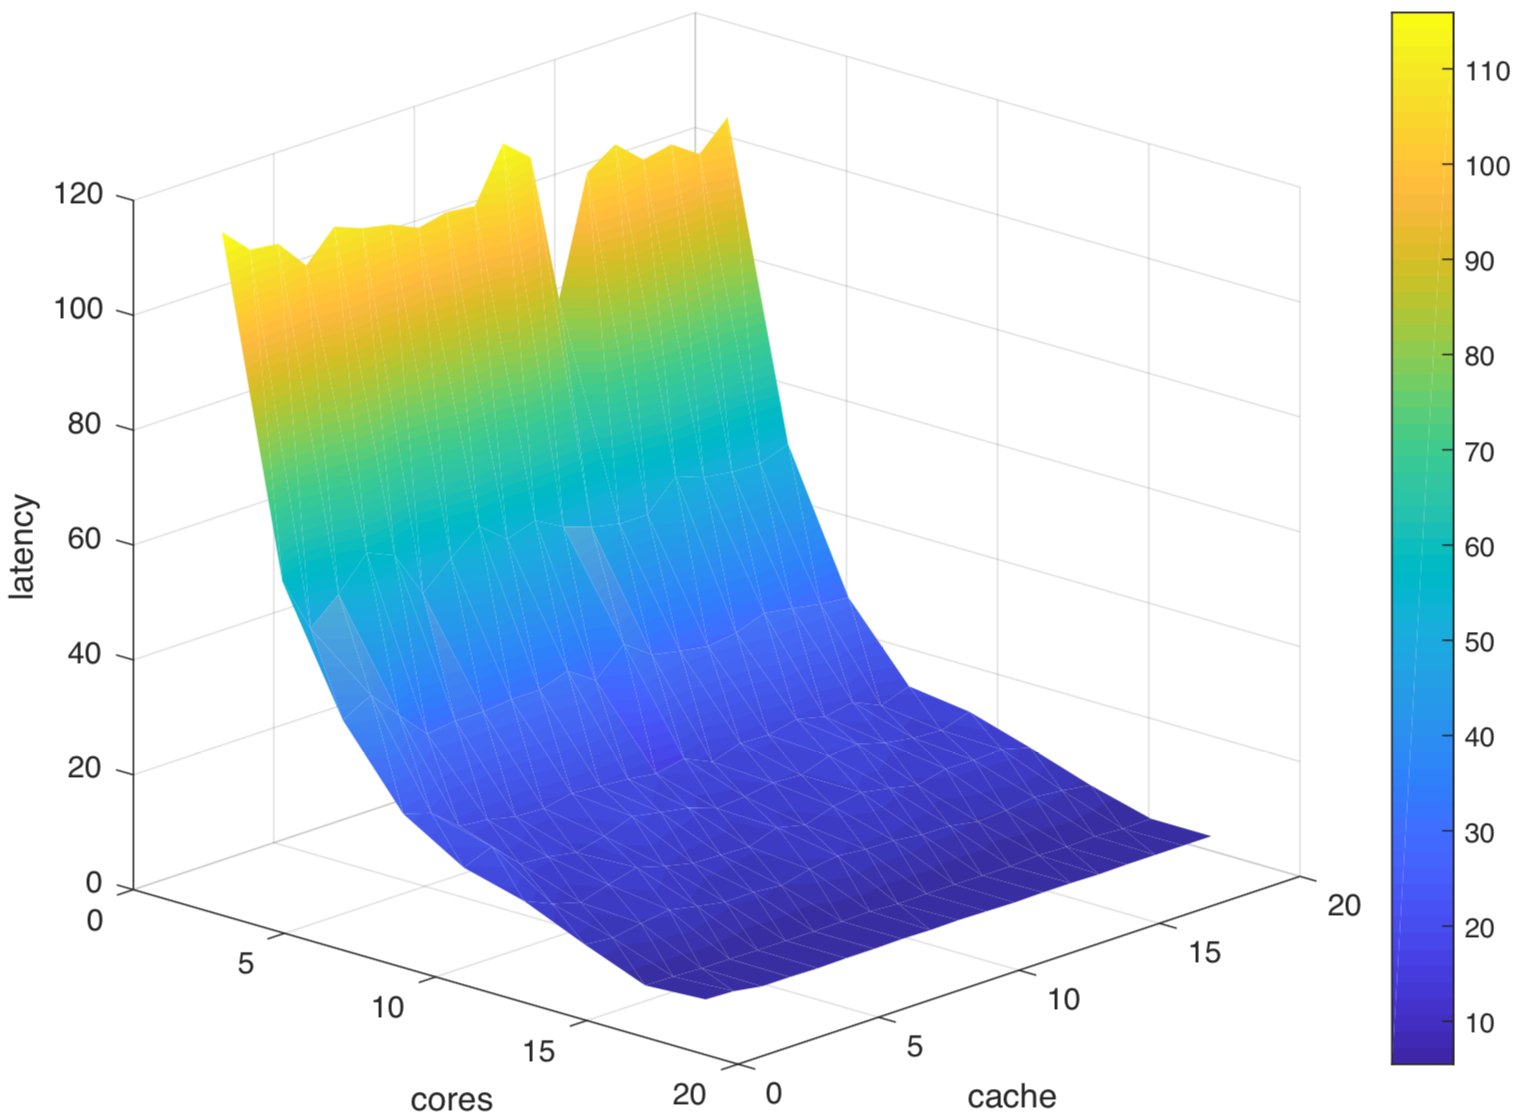
\includegraphics[height=5cm]{exp/datacache-profile.png}
    \captionof{figure}{单独执行}
  \end{subfigure}
  \hspace{1em}
  \begin{subfigure}{0.45\textwidth}
    \centering
    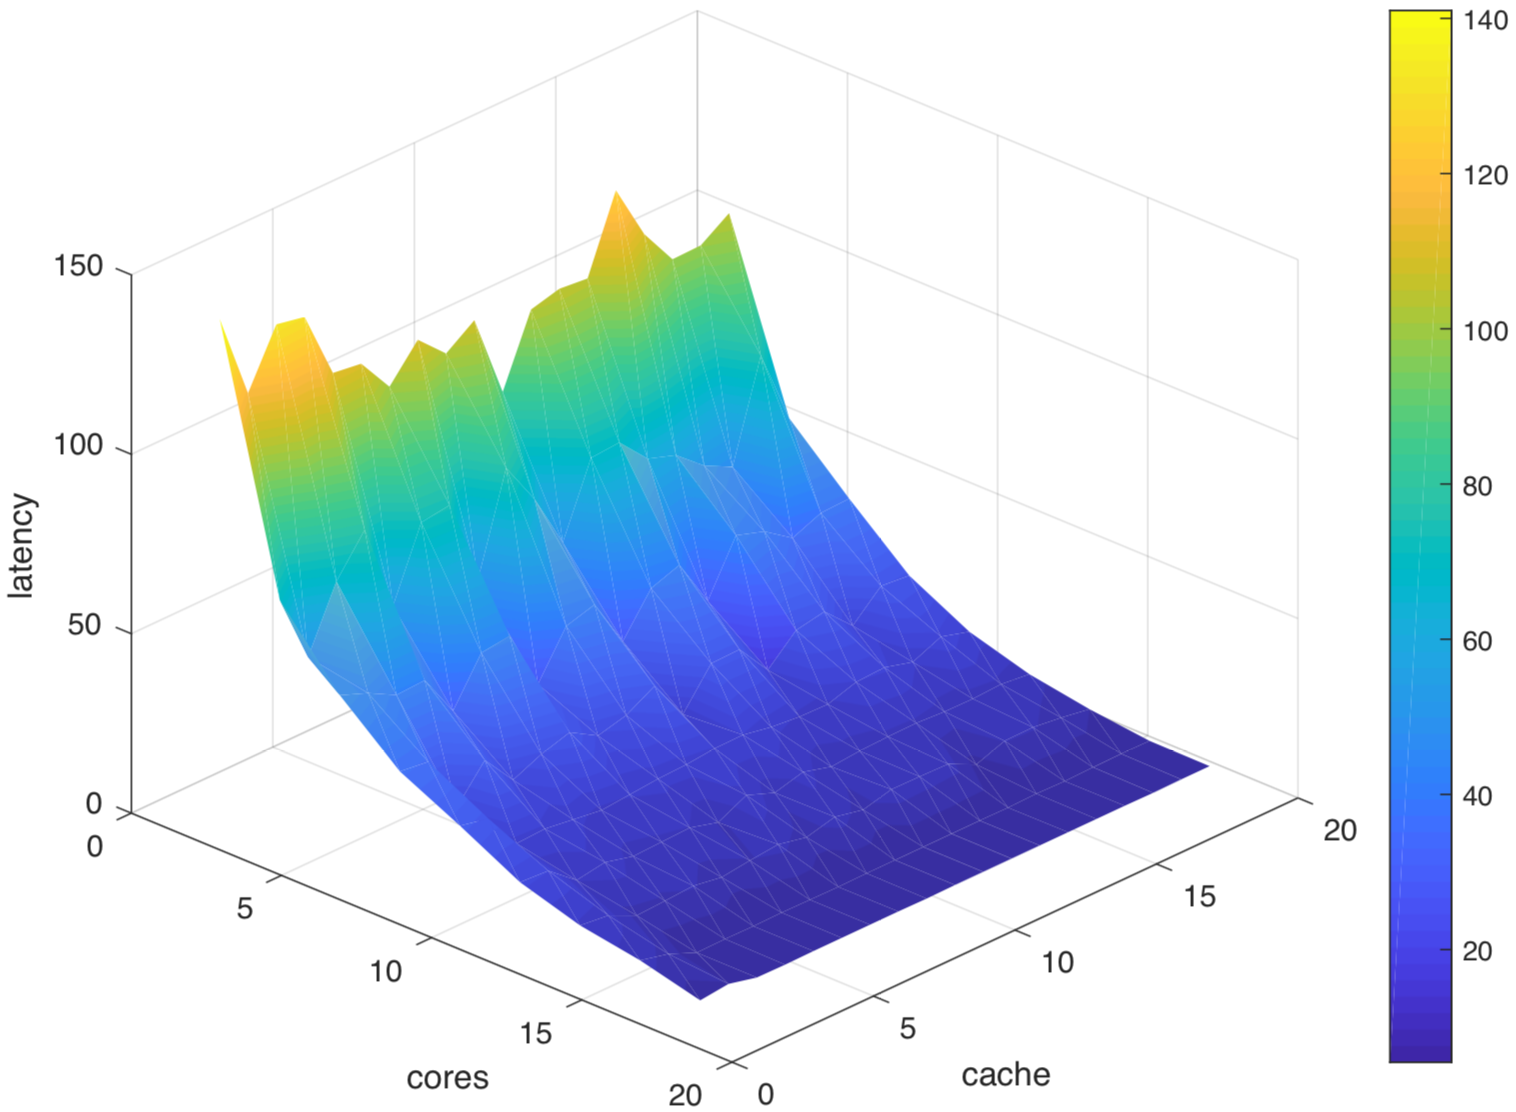
\includegraphics[height=5cm]{exp/datecache-profile-mix.png}
    \captionof{figure}{混合执行}
  \end{subfigure}
  \captionof{figure}{对象缓存的服务质量与服务器资源分配}
  \label{fig:data-cache-res}
\end{figure}


